%!TEX root = /Users/stevenmartell/Documents/CURRENT PROJECTS/iSCAM-trunk/fba/BC-herring-2011/WRITEUP/BCHerring2011.tex
\section{Bayesian prior for the dive survey spawn index proportionality constant $q$}\label{Appendix::q_prior}

\subsection{The process}

A Bayesian prior for the herring dive survey spawn index proportionality constant (q) is developed using a process that combines expert knowledge (in some cases best guesses) and data associated with factors influencing the prior.  The process, used to develop acoustic and trawl survey priors for New Zealand fisheries stock assessments \citep[e.g.,][]{CordueInPrep}, is comprised of the following steps: 

\begin{enumerate}
\item	List all factors affecting $q$.
\item	For each factor, determine the statistical distribution that best describes the uncertainty associated with that factor.  Where available, the distribution is based on data (not data that will be used in the assessment); otherwise it is based on expert knowledge. 
\item	The prior distribution for $q$ is estimated by integrating across the distributions for each factor.  This can be approximated by generating joint random samples from the distributions.
\item	Finally, a parametric model is fit to the resulting distribution of replicate random samples to approximate the $q$ prior.
\end{enumerate}

\subsection{Factors affecting $q$ and their distributions}
The factors that contribute to the spawn index $q$ prior include: the proportion of the total spawn that is surveyed; the amount of egg loss that occurs prior to the spawn survey; bias in the estimate of mean egg density; and drift in spawn survey observations over time. The distributions for each of these factors should reflect uncertainty in their average affect over years, not capture inter-annual variation in them. 

\subsubsection{Proportion of total spawn surveyed}
The proportion of the total spawn that is surveyed has a natural upper bound of 1, though its central tendency is not known. Reasons for not surveying herring spawns include non-detection (early or late in season or very deep and not observed) or lack of resources to conduct the survey.  For the latter case the spawns will be reported, and this occurrence is rare. The proportion of the total spawn that is not-detected is likely higher in more remote locations and when spawning abundance is low. With limited information, we assume a uniform distribution on 0.9 � 1.0 for the average proportion of total spawn surveyed. 

\subsubsection{Egg loss prior to survey}

This factor accounts for egg loss due to predation (seabirds, invertebrates, marine mammals) and translocation between the time of egg deposition and the spawn surveys.  The amount of egg loss prior to spawn surveys is determined by the daily egg loss rate and the number of days between a spawn and the subsequent survey. 

The herring egg loss literature, recently summarized by \cite[][their Appendix 7]{HayEggLoss}, is used to estimate a distribution for daily egg loss rates. All studies conducted on the west coast of North America that estimated total egg loss over the incubation period (or daily egg loss rates) were considered for inclusion in the egg loss rate distribution. Those criteria substantially reduce the available literature (Table \ref{AppendixC:Table3}). Egg loss estimates from the selected studies were standardized to instantaneous (daily) rates (Table \ref{AppendixC:Table4}). A normal distribution for the daily egg loss rate, based on the mean and standard deviation of the selected estimates, is assumed. 



The second component of the egg loss distribution is the average number of days between the spawn event and the surveys.  Information to inform the distribution of this factor was available in the B.C. herring spawn survey database.  Only �dive� survey records were selected, and numerous error checks imposed to remove erroneous data (Table \ref{AppendixC:Table4}).  For each spawn record, the number of days between the spawn event and subsequent survey was estimated as the difference between the mid-spawn date and the mid-survey date. The mean time between a spawn deposition event and the subsequent survey ranges from 6.4 to 9.2 days across the stock assessment regions (Table \ref{AppendixC:Table6}).  A normal distribution for the average time between egg deposition and surveys is assumed, based on the mean and standard deviation of the mean values for the stock assessment regions (mean=7.7; standard deviation =1.13). 


\subsubsection{Bias in mean egg density}

The equation predicting egg density from dive survey observations was calculated from field studies conducted through much of the B.C. coast in the mid 1980s.  These studies included diver observations of egg layers and percent cover by vegetation classes and subsequent laboratory egg counts of the observed quadrats.  While the egg density prediction equation is unbiased, the unexplained residual error is large and the error in the mean egg densities predicted at the stock assessment region/year level were often greater than expected based on the assumption of unbiased iid observations. To allow for potential bias in predicted mean egg density at the stock assessment region level, we assume a normal distribution for this factor with mean 1 and standard deviation 0.2.  

\subsubsection{Drift in dive survey observations}

The studies to calibrate field observations of herring spawns to egg density estimates were primarily conducted during the mid 1980s by research divers.  Since then, Fisheries Officers and subsequently research divers have conducted the coast wide herring spawn surveys. While there is considerable effort to ensure standardization of the surveys, it is possible that there has been drift in how observations are made.  There is no direct information on how survey observations may have changed over time, however Hay (in press) suggests that if drift has occurred it�s direction is to observations that result in lower density estimates (i.e. there has been an increase in �trace� observations.)  For now, we do not include this factor in calculating a prior distribution for the spawn survey $q$. 

Table \ref{AppendixC:Table1} summarizes the factors affecting the q prior and their assumed distributions.

\begin{table}[htdp]
\caption{Factors affecting the $q$ prior and their assumed distributions.}
\begin{center}
\begin{tabular}{llc}
\hline
Factor affecting the $q$ prior &	Distribution & Parameters of distribution\\
\hline
Proportion of total spawn surveyed ($p_i$)&Uniform &0.9�-1.0\\
%%
\multicolumn{3}{l}{Egg loss prior to survey:}\\
\multicolumn{1}{r}{Instantaneous daily egg loss rate ($Z_i$)}& Normal &Mean 0.0642  Std. dev 0.0187\\
\multicolumn{1}{r}{Days between spawn deposition and survey ($d_i$)}&Normal & Mean 7.7  Std. dev. 1.13\\
%%
Bias in mean egg density ($b_i$)&	Normal	&Mean 1  Std. dev.  0.2\\
\hline
\end{tabular}
\end{center}
\label{AppendixC:Table1}
\end{table}%



%%Table 1 roughly here
%%Table 2 roughly here


\subsection{Simulating the dive survey spawn index $q$}

Monte-Carlo simulations were conducted, randomly sampling from each factors� distribution.  The factors will operate independently so covariance structure does not need to be considered. For each of 10,000 replicates (i), a random draw was made for each factor to generate a point in the joint distribution for the $q$ prior ($\tilde{q}_i$): 
\[
\tilde{q}_i = p_i b_i \exp(-d_i Z_i)
\]

For the \iscam\ herring stock assessments, a lognormal prior for the spawn index $q$ is assumed (i.e., $\ln(q)$ is assumed normally distributed). The distribution of the simulated $\tilde{q}_i$  is reasonably approximated by a lognormal distribution (Figure \ref{AppendixC:fig1}). Means and standard deviations for the simulated  and the natural log of the $\tilde{q}_i$  are presented in Table \ref{AppendixC:Table2}

\begin{table}
\caption{Estimated means and standard deviations for the simulated q prior and natural log of the q prior.}\label{AppendixC:Table2}
\begin{center}
\begin{tabular}{lll}
\hline
 & $\tilde{q}_i$ & $\ln(\tilde{q}_i)$\\
 \hline
 Mean &0.587 & -0.569\\
 Std &0.155 & 0.274 \\
 \hline
\end{tabular}
\end{center}
\end{table}


\begin{figure}[!tbp]
	% Requires \usepackage{graphicx}
	\centering
	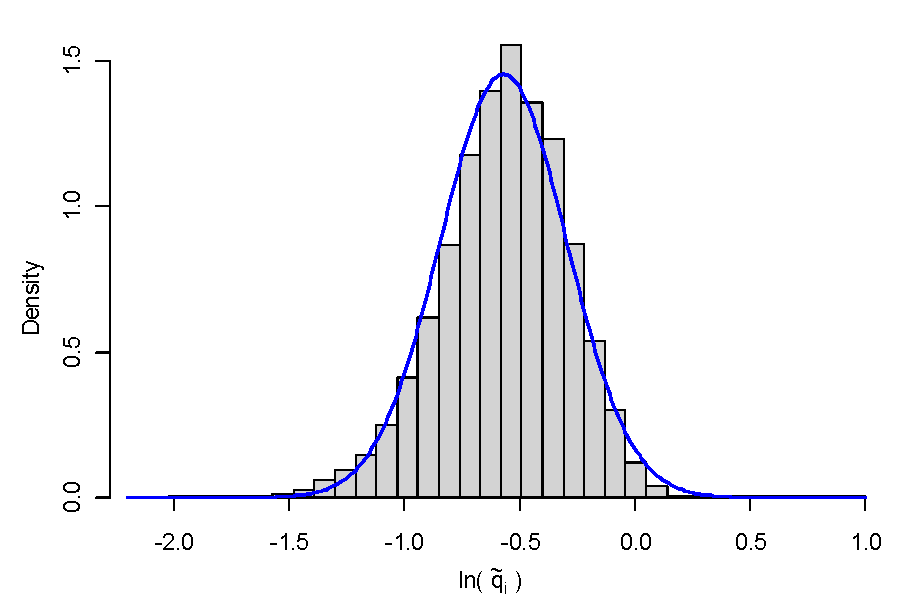
\includegraphics[width=\textwidth]{../FIGS/qprior.pdf}\\
	\caption{Distribution of the log of the simulated spawn index q estimates, overlaid with a normal distribution based on the mean and standard deviation of the simulated values.}\label{AppendixC:fig1}
\end{figure}


\begin{table}[htdp]
\caption{Summary of west coast North America herring egg loss literature.}
\begin{center}
\begin{tabular}{|p{0.65\textwidth}|p{0.35\textwidth}|}
\hline
\textbf{Study and summary of pertinent egg loss estimates:}&
\textbf{Rationale for inclusion/exclusion from prior estimation:}\\
\hline
\cite{bishop2001predation} &\\ Estimated 31\% of herring egg deposition was consumed by 5 species of birds (1994, Prince William Sound), based on a bioenergetics model. & Not included because study estimated only bird predation effect.\\
\hline
\cite{haegele1991egg} &\\
Estimated 58\% herring egg loss over 14 day incubation period (Lambert Channel 1989).  Bird and invertebrate predation accounted for 7.1\% egg loss; the remainder from physical removal and translocation could not be directly estimated.
&
Included because comprehensive B.C. study. \\
\hline
\cite{Haegele1989egg} & \\
Estimated 19.5\% egg loss from predation based on predator counts and consumption rates (birds and invertebrates).  From egg counts, total egg loss estimated at 68.8\% over a 14 day incubation period (their Table 3 egg loss equations).  Modelled changes in observations of egg layers over the incubation period:  egg layers on sea grasses= 2.17 � 0.07 (day); egg layers on filamentous algae= 3.47 � 0.13 (day).  Equations result in 45\% and 52\% decrease in egg layers over 14 days incubation period, respectively.
&
Included because comprehensive B.C. study. \\
\hline
\cite{outram1958magnitude}  & \\
Seabird predator exclusion study, West coast Vancouver Island (1951 � 1953).  Overall, estimated 39\% egg loss due to seabirds over the incubation period. Total egg loss over incubation period ranged from 56\% to 99\% (based on change in egg biomass for the control plots). Study was restricted to eelgrass beds.
&
Not included because study restricted to eel grass beds\\
\hline
\cite{palsson1984egg}  & \\
Estimated daily egg loss rates from 16.9\% to 51.8\% (positively correlated with egg density just after spawning).  Large predators account for 20\% to 50\% of daily egg loss.  Initial egg densities were very low, ranging from 400 to 80,000 eggs/m2 across 9 study sites.  Paulson�s thesis cites additional egg loss literature that is not included here because the studies generally focussed on a limited range of habitat types.
&
Not included because study egg densities were much lower than densities generally seen in B.C. spawns.\\
\hline
\cite{rooper1999habitat}& \\
Surveys conducted 1991, 1992, 1994 and 1995.  Depth is factor that best accounts for egg loss rates (higher egg loss in shallower waters).  Mean daily egg loss rates (Z) were (their Table 2):
\begin{itemize}
\item 1990 � 0.076
\item 1991 � 0.042
\item 1994 � 0.096
\item 1995 � 0.096 
\end{itemize}
Note that population was much lower in 1994 and 1995.
&
Comprehensive study in Prince William Sound.  Estimates for 1990 and 1991 only are included because population had crashed by 1994 and abundance was low.
\\
\hline
\end{tabular}
\end{center}
\label{AppendixC:Table3}
\end{table}



\begin{table}[htdp]
\caption{Estimates of the instantaneous daily egg loss rate (Z) from herring egg loss studies conducted in the Pacific Northwest. The Z estimates for the Haegele and Schweigert (1989, 1991) studies were calculated from their reported egg loss rates over the study period.}
\begin{center}
\begin{tabular}{llll}
\hline
Publication	&Study Location&	Year	&Z\\
\hline
Haegele \& Schweigert (1991) &	SoG &	1989	&0.056\\
Haegele \& Schweigert (1989)&WCVI&	1988&	0.083\\
Rooper et al. (1999)&	PWS	&1991	&0.076\\
Rooper et al. (1999)&	PWS	&1992	&0.042\\
\hline
& & Mean & 0.0642\\
& & Std & 0.0187\\
\hline
\end{tabular}
\end{center}
\label{AppendixC:Table4}
\end{table}%

\begin{table}[htdp]
\caption{default}
\begin{center}
\begin{tabular}{lc}
\hline
Selection criterion	 &Number of Records\\
\hline
Total dive survey records (1985-2010)	&3457\\ \hline
Spawn and survey start/end dates completed &	3188\\ \hline
End spawn date $\leq$ start spawn date &\\
End spawn date � start spawn date $<$ 20 &\\
Survey days $\leq$ 14	3130 &  3130\\ \hline
End spawn date-end survey date$\leq$ 2 &\\
End survey date- end spawn date $<$ 20&	3074\\
\hline
\end{tabular}
\end{center}
\label{AppendixC:Table5}
\end{table}%


\begin{table}[htdp]
\caption{Average number of days between spawn deposition and spawn survey by stock assessment region and year.}
\begin{center}
\begin{tabular}{llllllll}
\hline
Year&A2W&HG&PRD&CC&SoG&WCVI&A27\\
\hline
1985&& & & &5.2&6.6&8.8\\
1986& & &6.0&5.5&5.8&9.2&2.2\\
1987& & & & &10.6& & \\
1988& &7.4&11.2&8.3&11.0&8.2& \\
1989& &8.2&10.8&5.8&14.5&8.6&10.7\\
1990&8.9&12.2&8.3&7.9&12.8&7.6&7.8\\
1991&10.5&5.9&7.5&11.0&12.4&9.2&2.3\\
1992&3.6&0.1&6.6&10.0&8.1&9.4&5.7\\
1993&12.2&9.3&4.9&9.1&13.1&7.6&16.8\\
1994&4.8&12.2&10.8&8.7&12.8&6.2& \\
1995& &10.3&6.1&7.9&9.3&6.4&11.1\\
1996& &7.9&5.7& &10.2&4.5&7.9\\
1997& &8.6&10.3&6.1&9.4&7.5&2.8\\
1998&10.5&13.3&5.5&12.4&10.4&6.4&4.2\\
1999& &10.0&8.1&6.4&8.0&4.9& \\
2000&6.5&10.8&10.8&7.4&8.8&6.1&6.9\\
2001&9.0&7.4&8.3&6.8&8.0&6.9&3.8\\
2002&6.5&9.0&5.7&5.6&9.9&5.5&2.3\\
2003& &7.5&6.2&5.0&9.5&7.0&7.3\\
2004&8.6&14.0&8.2&4.1&9.5&7.1&8.2\\
2005&6.3&9.4&8.8&9.2&5.8&5.1&3.3\\
2006& & &7.6&6.5&11.7&3.1&5.8\\
2007& &6.0&10.8&0.7&9.3&3.4& \\
2008& &7.4&7.2&4.3&9.5&3.8&2.0\\
2009&5.3&6.0&9.6&5.3&4.2&5.5&5.6\\
2010& & & & &7.1&5.2& \\
\hline
Mean&7.8&8.7&8.3&6.8&9.2&6.6&6.4\\
\hline
\end{tabular}
\end{center}
\label{AppendixC:Table6}
\end{table}%


